\clearpage
\myparagraph{\olly}
\index{\olly}

\RU{Попробуем этот пример в}\EN{Let's try this example in} \olly.
\RU{Входное значение функции}\EN{The input value of the function} (2) \RU{загружается в}\EN{is loaded into} \EAX: 

\begin{figure}[H]
\centering
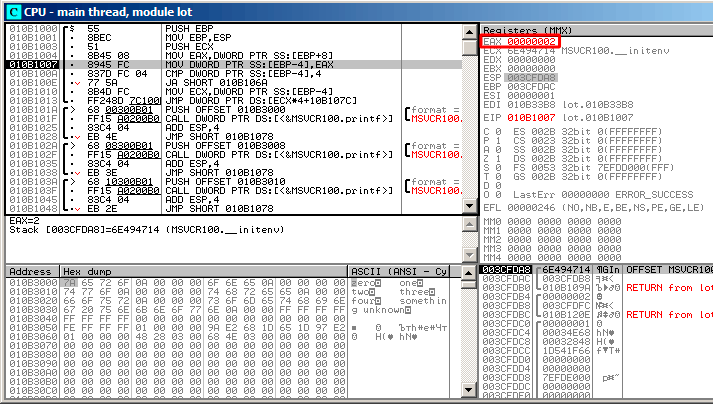
\includegraphics[scale=\FigScale]{patterns/08_switch/2_lot/olly1.png}
\caption{\olly: \RU{входное значение функции загружено в}\EN{function's input value is loaded in} \EAX}
\label{fig:switch_lot_olly1}
\end{figure}

\clearpage
\RU{Входное значение проверяется, не больше ли оно чем}\EN{The input value is checked, is it bigger than} 4? 
\RU{Нет, переход по умолчанию (\q{default}) не будет исполнен}\EN{If not, the \q{default} jump is not 
taken}:
\begin{figure}[H]
\centering
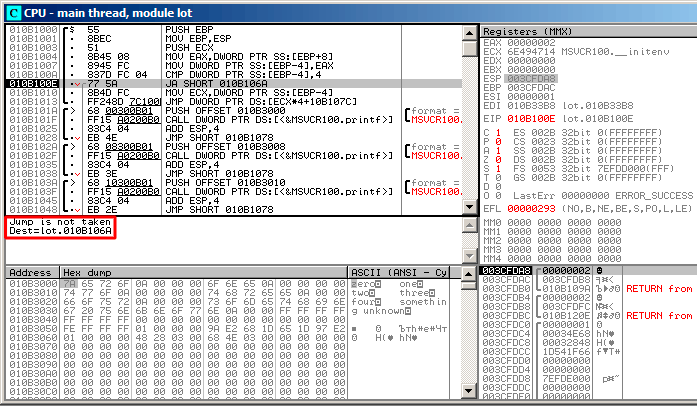
\includegraphics[scale=\FigScale]{patterns/08_switch/2_lot/olly2.png}
\caption{\olly: 2 \RU{не больше чем}\EN{is no bigger than} 4: \RU{переход не сработает}\EN{no jump is taken}}
\label{fig:switch_lot_olly2}
\end{figure}

\clearpage
\RU{Здесь мы видим}\EN{Here we see a} jumptable:

\begin{figure}[H]
\centering
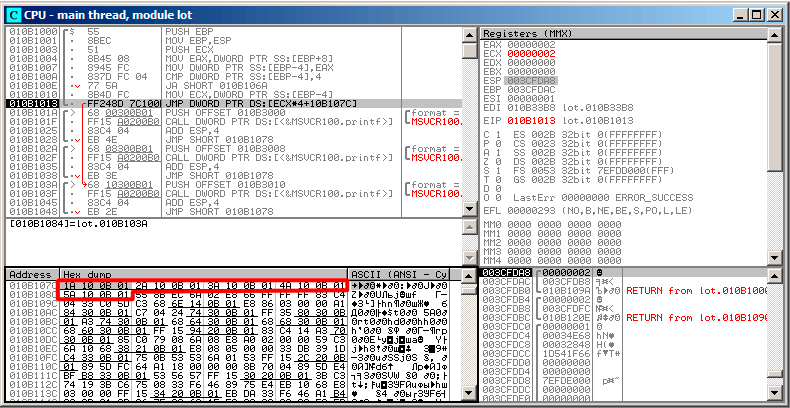
\includegraphics[scale=\FigScale]{patterns/08_switch/2_lot/olly3.png}
\caption{\olly: \RU{вычисляем адрес для перехода используя}\EN{calculating destination address using} jumptable}
\label{fig:switch_lot_olly3}
\end{figure}

\RU{Кстати, я щелкнул по}\EN{Here I've clicked} \q{Follow in Dump} $\rightarrow$ \q{Address constant}, 
\RU{так что теперь jumptable видна в окне данных}\EN{so now we see the jumptable in the data window}. 
\RU{Это 5 32-битных значений}\EN{These are 5 32-bit values}\footnote{\EN{They are underlined by \olly because
these are also FIXUPs}\RU{Они подчеркнуты в \olly, потому что это также и FIXUP-ы}: \myref{subsec:relocs}, 
\RU{мы вернемся к ним позже}\EN{we are going to come back to them later}}.
\ECX \RU{сейчас содержит}\EN{is now} 2\RU{, так что второй элемент (считая с нулевого) таблицы
будет использован}\EN{, so the second element (counting from zero) of the table is to be used}.
\RU{Кстати, можно также щелкнуть}\EN{It's also possible to click} \q{Follow in Dump} $\rightarrow$ 
\q{Memory address} \AndENRU \olly 
\RU{покажет элемент, который сейчас адресуется в инструкции \JMP}%
\EN{will show the element addressed by the \JMP instruction}. 
\RU{Это}\EN{That's} \TT{0x010B103A}.

\clearpage
\RU{Переход сработал и мы теперь на}\EN{After the jump we are at} \TT{0x010B103A}: 
\RU{сейчас будет исполнен код, выводящий строку}\EN{the code printing} \q{two}\EN{ will now be executed}:

\begin{figure}[H]
\centering
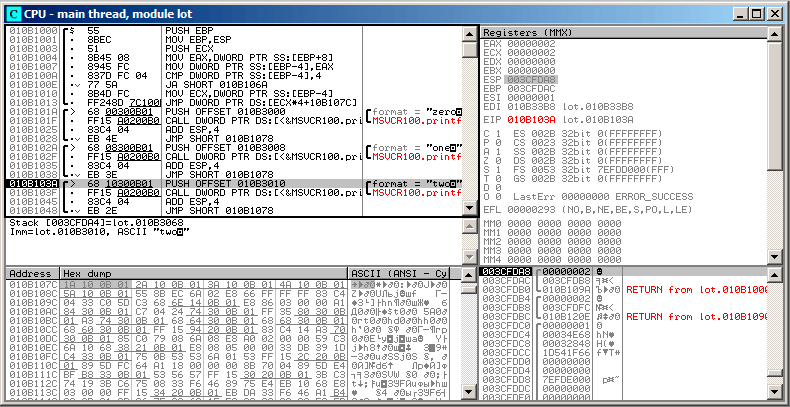
\includegraphics[scale=\FigScale]{patterns/08_switch/2_lot/olly4.png}
\caption{\olly: \RU{теперь мы на соответствующей метке}\EN{now we at the} \IT{case:}\EN{ label}}
\label{fig:switch_lot_olly4}
\end{figure}
